\documentclass[12pt]{article}
\usepackage{amsmath}
\usepackage{amssymb}
\usepackage{color}
\usepackage{tikz}
\usetikzlibrary{matrix}

\begin{document}

\begin{center}
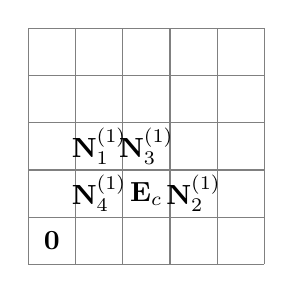
\begin{tikzpicture}[scale=0.6]
    \draw [gray] (0,0) grid (5,5);
    \node at (0.5,0.5) {$\mathbf{0}$};
    \node at (1.5,1.5) {$\mathbf{N}^{(1)}_{4}$};
    \node at (2.5,1.5) {$\mathbf{E}_{c}$};
    \node at (3.5,1.5) {$\mathbf{N}^{(1)}_{2}$};
    \node at (1.5,2.5) {$\mathbf{N}^{(1)}_{1}$};
    \node at (2.5,2.5) {$\mathbf{N}^{(1)}_{3}$};
\end{tikzpicture}
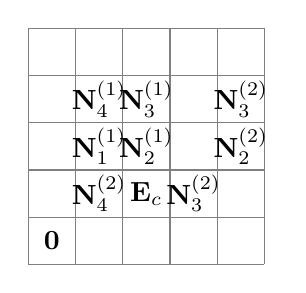
\begin{tikzpicture}[scale=0.6]
    \draw [gray] (0,0) grid (5,5);
    \node at (0.5,0.5) {$\mathbf{0}$};
    \node at (1.5,1.5) {$\mathbf{N}^{(2)}_{4}$};
    \node at (2.5,1.5) {$\mathbf{E}_{c}$};
    \node at (3.5,1.5) {$\mathbf{N}^{(2)}_{3}$};
    \node at (1.5,2.5) {$\mathbf{N}^{(1)}_{1}$};
    \node at (2.5,2.5) {$\mathbf{N}^{(1)}_{2}$};
    \node at (4.5,2.5) {$\mathbf{N}^{(2)}_{2}$};
    \node at (1.5,3.5) {$\mathbf{N}^{(1)}_{4}$};
    \node at (2.5,3.5) {$\mathbf{N}^{(1)}_{3}$};
    \node at (4.5,3.5) {$\mathbf{N}^{(2)}_{3}$};
\end{tikzpicture}
\end{center}

Illustrations of our recursive encryption algorithm. There is a two-dimensional plane with $3 \times 3$ pixels, where multiple events $\mathbf{E}_c$ are triggered in the center, and the rest of the pixels are on the mask for synthetic noise. In the $1$st layer of the recursion (left), the algorithm synthesizes the noise $\mathbf{N}^{(1)}_i (i=1,2,3,4)$ in $4$ spatial neighbors horizontally/vertically adjacent to $\mathbf{E}_c$, where $|\mathbf{N}^{(1)}_i| = |\mathbf{E}_c|$. The resulting $\mathbf{N}^{(1)}_i \cup \mathbf{E}_c$ will be the input of the $2$nd layer of the recursion (right). The algorithm, which is blind to $\mathbf{N}^{(1)}_i$ and $\mathbf{E}_c$, synthesizes the noise $\mathbf{N}^{(2)}_i (i=1,2,3,4)$ based on the adjacent events.

\end{document}